%%%%%% CMB-S4 Introduction %%%%%%%%%%%%%%%%
 
\chapter{Exhortations}
\label{chap:intro}

%%%%%%%%%%%%%%%%%%%%%%%%%%%%%%%%%%%%%%%%%%%%%%%



%%%

\begin{center}
{\small \it (send feedback on this chapter to \href{mailto:jc@kicp.chicago.edu}{jc@kicp.chicago.edu})}
\end{center}

Fourteen billion years ago, in the first fraction of a second of our universe's existence, the most extreme high-energy physics experiment took place. Our ability to use the cosmic microwave background (CMB) to investigate this fantastic event, at energy scales a trillion times higher than can be obtained at the CERN, is at the very core of our quest to understand the fundamental nature of space and time and the physics that drive the evolution of the universe. 

The CMB allows direct tests of models of the quantum mechanical origin of all we see in the universe. Subtle correlations in its anisotropy imparted by the interplay of gravitational and quantum physics at high energies contain information on the unification of gravity and quantum physics. Separately, correlations induced on the background at later times encode details about the distribution of all the mass, ordinary and dark, in the universe, as well as the properties of the neutrinos, including the number of neutrino species and types, and their still unknown masses. 

Here we describe the scientific case for the next generation ground-based cosmic microwave background experiment, CMB-S4, consisting of dedicated telescopes at the South Pole, the high Chilean Atacama plateau and possibly a northern hemisphere site, all equipped with new superconducting cameras that will provide a dramatic leap forward in cosmological studies, crossing critical thresholds in testing inflation, the number and masses of the neutrinos or the existence of other `dark radiation', providing precise constraints on the nature of dark energy, and testing general relativity on large scales. 

Through the efforts of the CMB experimental groups over the last decade, the technologies needed for CMB-S4 are now in place. There are, however, considerable technical challenges presented by the required scaling up of the instrumentation as well as by the scope and complexity of the data analysis and interpretation.  CMB-S4 will require: scaled up superconducting detector arrays with well understood and robust material properties and processing techniques; high throughput mm-wave telescopes and optics with unprecedented precision and rejection of systematic contamination; full characterization of astronomical foreground emission; large cosmological simulations and theoretical modeling with accuracies yet to be achieved; and computational methods for extracting minute correlations in massive, multi-frequency data sets contaminated by noise and a host of known and unknown signals. 

The purpose of this document is to set the scientific goals for CMB-S4 and (eventually) the instrumental configuration required to achieve them.  This is of course an iterative process, involving detailed simulations as well as cost considerations. So, at this time the Science Book is a working document with this first iteration focused primarily on defining the possible science reach in several areas, along with the simulations needed to refine the science case and set the specifications of the needed measurements. This will set the stage for defining the instrument  in the next iteration of the Science Book. 

In this chapter we set out the overarching goals for CMB-S4, which are then refined in later chapters.  We start with a brief history and the current status of CMB measurements. 


\section{Brief History and Current Status of CMB measurements}
\label{sec:background}

From its discovery 50 years ago, measurements of the cosmic microwave background (CMB) have led to spectacular scientific insights into the fundamental workings of space and time, from the quantum mechanical origin of the Universe at extremely high energies in the first moments of the Universe, through the growth of structure and the emergence of the dark energy that now dominates the energy density of the Universe. Studies of the CMB connect physics at the smallest scales and highest energies with the largest scales in the Universe, roughly 68 orders of magnitude in length scale. They connect physics at the earliest times to the structure that surrounds us now, over 52 magnitudes in time scale. 

The deep connections of CMB studies and particle physics predate the discovery of the background, going back to the 1940s when Alpher and Gamow were considering a hot, dense, early Universe as a possible site for nucleosynthesis. To produce the
amount of helium observed in the local Universe, they concluded there
had to be about $10^{10}$\ thermal photons for every nucleon. Alpher and Herman subsequently predicted that this background of photons would persist to the present day as a thermal bath at a few degrees Kelvin.

The continuing, remarkably successful, story of CMB studies is one driven by the close interplay of theory and phenomenology with increasingly sensitive and sophisticated experiments. The high degree of isotropy of the CMB across the sky, to a part of one in a hundred thousandth, led to the theory of inflation and cold dark matter in the 1980's. It was not until 1992 that COBE discovered the anisotropy, and pinned the level of anisotropy for the following higher angular resolution measurements to characterize. In 2006 the COBE measurements of the background anisotropy and its black-body spectrum were recognized with the second Nobel Prize in physics; the first was awarded in 1978 to Penzias and Wilson for the discovery of the CMB.  In the decade after the COBE results, measurements with ground and balloon-based instruments revealed the acoustic peaks in the CMB angular power spectrum, which showed that the Universe was geometrically flat in accordance with predictions of inflation and provided strong support for contemporary claims for an accelerating Universe based on observations of type Ia supernovae (SNe), which were recognized with the 2011 Nobel Prize in physics. The early anisotropy measurements also provided an estimate of the universal baryon density and found it to be in excellent agreement with the level estimated at $t \sim 1$ second by big bang nucleosynthesis (BBN) calculations constrained to match the observed elemental abundances. The CMB measurements also clearly showed that dark matter was non-baryonic. The polarization anisotropy was discovered ten years after COBE at the level predicted from temperature anisotropy measurements. The now standard $\Lambda$CDM cosmological model was firmly established.

Two CMB satellites have mapped the entire sky over the last 15 years, first WMAP with moderate angular resolution (as fine as 12 arcminutes), followed by Planck with resolution as fine as 5 arcminutes. Higher-resolution maps of smaller regions of the sky have been provided by ground-based experiments, most notably by the 10m South Pole Telescope (SPT) and the 6m Actacama Cosmology Telescope. The primary CMB temperature anisotropy is now well characterized through the damping tail, i.e., to multipoles $\ell \sim 3000$, and secondary anisotropies have been measured to multipoles up to  $10,000$.   The $\Lambda$CDM model continues to hold up stunningly well, even as the precision of the CMB determined parameters has increased substantially. Inflationary constraints include limits on curvature constrained to be less than 3\% of the energy density, non-Gaussian fluctuations limited to $f_{NL} < 10$, and 
the predicted small departure from pure scale invariance of the primordial fluctuations detected at 5-sigma confidence. Also of interest to particle physics, the effective number of light relativistic species (i.e., neutrinos and any yet identified ``dark radiation") is shown to be within one sigma of $\neff = 3.046$, the number predicted by BBN.  The sum of the masses of the neutrinos is found to be less than 0.6 eV. Dark matter is shown to be non-baryonic at $> 40$ sigma. Early dark energy models are highly constrained as are models of decaying dark matter. 

There remains much science to extract from the CMB, including: 1) using CMB B-mode polarization to search for primordial gravitational waves to constrain the energy scale of inflation and to test alternative models, and to provide insights into quantum gravity; 2) obtaining sufficiently accurate and precise determinations of the effective number of light relativistic species (dark radiation) to allow independent and rigorous tests of BBN as well as our understanding of the evolution of the Universe at $t = 1$\ sec; 3) a detection of the sum of the neutrino masses, even at the minimum mass allowed by oscillation experiments and in the normal hierarchy; 4) using secondary CMB anisotropy measurements to provide precision tests of dark energy through its impact on the growth of structure; and 5) testing general relativity and constraining alternate theories of gravity on large scales.

Currently the best cosmological constraints come from analyzing the combination of primary and secondary CMB anisotropy measurements with other cosmological probes, such as baryon acoustic oscillations (BAO) and redshift distortions, weak lensing, galaxy and galaxy cluster surveys, Lyman-alpha forest measurements, local determinations of the Hubble constant, observations of type Ia SNe, and others. The CMB primary anisoptropy measurements provide highly complementary data for the combined analysis, in particular by providing a precision measurement of the Universe at $z = 1100$, which will provide a precise prediction for measurements of the late time Universe for any cosmological model and set of parameters -- the Hubble constant, BAO scale, and the normalization of the present day matter fluctuation spectrum being excellent examples. Secondary CMB measurements provide late-time probes directly from the CMB measurement, e.g., CMB lensing, the SZ effects and SZ cluster catalogs, which will provide critical constraints on the standard cosmological models and extensions to it. The cosmological reach of future cosmological surveys at all wavelengths will be greatly extended by their joint analyses with secondary CMB anisotropy measurements. 


\section{Science reach of CMB-S4}
\label{sec:science}

CMB-S4 should be the definitive ground-based CMB project. The key science topics it should cover, and cover well, are

\begin{enumerate}

\item{Inflation:
CMB-S4 should make the definitive B-mode measurement at degree angular scales, where the signal from inflationary gravitational waves is predicted to have a local peak. This measurement will require multiple bands to untangle the foregrounds and sensitivity at degree through arcminute angular scales to obtain the required CMB lensing and E-mode measurements for ``de-lensing.'' If it can be demonstrated that  foregrounds and atmospheric noise can be mitigated at very large scales, CMB-S4 should also target the predicted peak at angular scales of tens of degrees. At these largest scales, CMB-S4, balloon and satellite mission would be highly complementary.

With these B-mode measurements, CMB-S4 should constrain the tensor-to-scalar ratio $r$ well enough to answer whether or not large-scale, slow-roll, single-field inflation models are viable ($r \gtrsim 0.01$) with high significance. In the absence of a detection, CMB-S4 should be able to rule out at high significance all models that naturally explain the observed value of the scalar spectral index, setting a rough sensitivity target of $\sigma(r)=0.001$.

If $r$ is detected before or by CMB-S4, then CMB-S4 should provide a robust, cosmic-variance-limited measure of its value (requiring a large-area survey) and set the best possible constraints on $n_t$ (requiring an ultra deep survey). 

CMB-S4 should provide the polarization data to test predictions of models that attempt to explain the low-ell temperature power spectrum ``anomalies'' that may offer clues to inflation. It will be particularly important to achieve accurate $20 < \ell < 100$ E-mode measurements.

 CMB-S4 will also extend the lever arm for measuring the scalar spectral index $n_s$, particularly in the EE spectrum. While foregrounds in the TT spectrum limit even futuristic measurements to $\ell \sim 4000$, the very low level of polarized foregrounds at high $\ell$ indicate that measurements of the primary E-mode spectrum could be extended to higher $\ell.$

The CMB-S4 data set should be the definitive data set with which any model for the origin of the primordial fluctuations, be it inflationary or an alternative theory, must be consistent with to be viable.
}

\item{Neutrinos and light relativistic species:

There are two primary areas in which CMB-S4 will provide interesting constraints on neutrino physics and the presence of new light particles.


a) The first is the effective number of light relativistic species, \neff. This is uniquely probed by the CMB and provides a critical constraint on any model for the neutrinos and their interactions or of other light dark-sector relics. It is a highly complementary probe to BBN and to sterile neutrino models.  Finding consistency with $\neff = 3.046$ at a precision of 0.020 would be an exciting and fundamental achievement linking particle physics and our understanding of the evolution of the first seconds of the Universe. Finding a departure from 3.046 would be even more exciting. %Recent work indicates that CMB-S4 with arc minute sensitivity may allow even tighter \neff\ constraints. 

b) The second is the constraint on the sum of the masses of the neutrinos, $\Sigma m_\nu$. Here CMB-S4 will achieve %$\sigma(\Sigma m_\nu) = 16$~meV (with DESI BAO prior), with the CMB sensitivity coming primarily through CMB lensing. This will lead to 
a definite detection of neutrino mass, even at the minimum mass and the normal hierarchy. The sensitivity of cosmic probes to the sum of the masses is unique and complementary to terrestrial neutrino experiments.
 }

\item{Dark Energy and Gravity:

 The CMB can be used to investigate dark energy through growth-of-structure tests using CMB lensing and SZ clusters, and through testing Gravity on large scales by exploiting the kinematic SZ effect to measure the momentum field and large-scale flows. The power of these probes is amplified by combining CMB-S4 data with galaxy surveys and Lyman alpha surveys, such as DESI, LSST, Euclid and WFIRST.

 a) CMB lensing measurements from CMB-S4 will provide high-fidelity projected mass maps that will be cross-correlated with optical survey maps. This will increase the reach and precision of the dark energy constraints, as well as provide independent checks. %Papers in the literature have quantified the dark energy figure of merit (FOM) improvement of various projects with the addition of CMB lensing. Simulations need to be done to quantify the projected improvements with CMB-S4.

 b) As noted by the dark energy task force (DETF), measurements of the evolution of galaxy cluster abundance have the highest raw sensitivity of any dark energy probe. The key to exploiting this sensitivity is controlling systematic uncertainties, primarily in the estimation of cluster masses. CMB-S4 will be revolutionary in that it is expected to be able to calibrate the mass scaling to better than 1\% through CMB lensing. This coupled with a low mass threshold will enable CMB-S4 to identify of order 100,000 clusters, probe the growth of structure to redshifts beyond $z \sim 2.5$, and realize the full potential of galaxy clusters as a probe of dark energy.  In combination with other Stage-IV baryon acoustic oscillation, supernova, and weak lensing surveys, a Stage-IV cluster survey similar to CMB-S4 should improve the overall dark energy figure of merit to approximately 1250, nearly a factor of two above what can be achieved without clusters. 

 c) Testing GR on large scales is important for our understanding of dark energy and the underlying workings of space and matter in general.  The kinematic SZ effect allows measurement of the peculiar velocity (departure from Hubble flow) of structures. By measuring the differences in kSZ between pairs of clusters with known redshifts (a synergy of CMB-S4 and optical surveys), gravity can be tested on scales of 100~Mpc and larger. In this way, CMB-S4 paired with a Stage-IV spectroscopic survey would improve constraints on the growth rate predicted by general relativity by a factor of two.
 }

\end{enumerate}

Lastly it would be an oversight not to point out the obvious: there is only one CMB sky. It holds a wealth of information on fundamental physics and the origin and evolution of the Universe. While we have learned a great deal from CMB measurements, including discoveries that have pointed the way to new physics, we have only begun to tap the information contained in CMB polarization, CMB lensing and secondary effects. CMB-S4 should be designed to maximize discovery space by producing high-fidelity maps. 

\section{From science goals to CMB-S4 design}


\subsection{Conceptual design of CMB-S4}

The science goals discussed above leads to a rough conceptual design of CMB-S4, which we describe below.

\subsubsection{Sensitivity and detector count}

\begin{figure}[t]
\centering 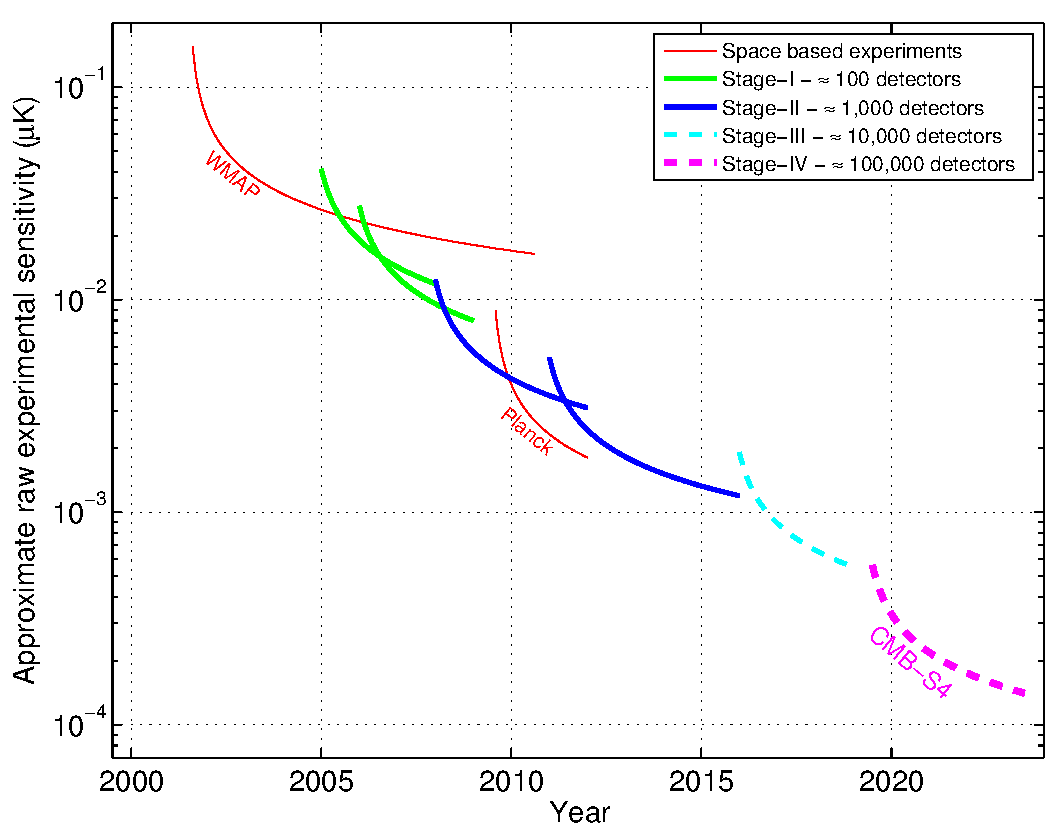
\includegraphics[width=0.6\textwidth]{Intro/expt_progress.pdf}
\caption{Plot illustrating the evolution of the raw sensitivity of CMB
  experiments, which scales as the total number of
  bolometers. Ground-based CMB experiments are classified into Stages
  with Stage II experiments having $O$(1000) detectors, Stage III
  experiments having $O$(10,000) detectors, and a Stage IV experiment
  (such as \cmbexp) having $O$(100,000) detectors. Figure from Snowmass  CF5
  Neutrino planning document.}
\label{fig:expt_progress-intro}
\end{figure}

The sensitivity of CMB measurements has increased enormously since Penzias and Wilson's discovery in 1965, following a Moore's Law like scaling, doubling every roughly 2.3 years. Fig.~\ref{fig:expt_progress-intro} shows the sensitivity of recent experiments as well as expectations for upcoming Stage 3 experiments, characterized by order 10,000 detectors on the sky, as well as the projection for a Stage 4 experiment with order 100,000 detectors. To obtain many of the CMB-S4 science goals requires of order $1~\mu$K arcminute sensitivity over roughly half of the sky, which for a four-year survey requires of order 500,000 CMB-sensitive detectors. 

To maintain the Moore's Law-like scaling requires a major leap forward, a phase change in the mode of operation of the ground based CMB program.  Two constraints drive the change:  1) CMB detectors are background-limited, so more pixels are needed on the sky to increase sensitivity; and 2) the pixel count for CMB cameras are nearing saturation.  Even using multichroic pixels and wide field of view optics, CMB telescopes are expected to field only tens of thousands of polarization detectors, far fewer than needed to meet the CMB-S4 science goals. 

CMB-S4 thus requires multiple telescopes, each with a maximally outfitted focal plane of pixels utilizing superconducting, background limited, CMB detectors. To achieve the large sky coverage and to take advantage of the best atmospheric conditions, the South Pole and the Chilean Atacama sites are baselined, with the possibility of adding a new northern site to increase sky coverage to the entire sky not contaminated by the Galaxy.

\subsubsection{Inflationary B-modes: low $\ell$ sensitivity, foregrounds and atmospheric noise mitigation}

At the largest angular scales (low $\ell$)---the angular scales that must be measured well to pursue inflationary B-modes as well as critical tests of the E-mode polarization---the CMB polarization anisotropy is highly contaminated by foregrounds. Galactic synchrotron dominates at low frequencies and galactic dust at high frequencies, as recently shown by the Planck and Planck/BICEP/KECK polarization results. Multi-band polarization measurements are required to distinguish the primordial polarized signals from the foregrounds. 

Adding to the complexity of low multipole CMB observations is the need to reject the considerable atmospheric noise contributions over the large scans needed to extract the low 
$\ell$ polarization. While the spatial and temporal fluctuations of the atmosphere are not expected to be polarized, any mismatches in the polarized beams or detector gains will lead to T-P leakage. These issues can be mitigated by including additional modulations into the instrument design, such as bore-sight rotation or modulation of the entire optics with a polarization modulation scheme in front of the telescope. Implementing such modulations is easier for small telescopes, although they could in principle be implemented on large telescopes as well. The cost of a small aperture telescope is dominated by the detector array, making it feasible to deploy multiple telescopes each optimized for a single band, or perhaps multiple bands within the relatively narrow atmosphere windows.

It is therefore an attractive option for CMB-S4 to include dedicated small aperture telescopes for pursuing low-$\ell$ polarization. The default plan for CMB-S4 is to target the recombination bump, with E-mode and B-mode polarization down to $\ell \sim 20$. If Stage 3 experiments demonstrate that it is feasible to target the reionization bump from the ground, those techniques may be incorporated into CMB-S4. More likely, however, this is the $\ell$ range for which CMB-S4 will be designed to be complementary to balloon-based and satellite based measurements. 

\subsubsection{Neutrinos, light relics, and dark energy: high $\ell$ sensitivity}

At the highest angular resolution (high $\ell$)--- the angular scales needed for de-lensing the inflationary B-modes, constraining \neff\ and $\Sigma m_\nu$,  investigating dark energy and performing gravity tests with secondary CMB  anisotropy ---the CMB polarization anisotropy is much less affected by both foregrounds and atmospheric noise. In fact, it should be possible to measure the primary CMB anisotropy in E-mode polarization to multipoles significantly higher than is possible in TT, thereby extending the lever arm to measure the spectral index and running of the primordial scalar (density) fluctuations. CMB lensing benefits from $\ell_{max}$ of order 5000 and secondary CMB measurements are greatly improved with $\ell_{max}$ of order 10,000 and higher, requiring large-aperture telescopes with diameters of several meters. Owing to the steep scaling of telescope cost with aperture diameter, it is likely not cost-effective to consider separate large aperture telescopes each optimized for a single frequency band. 

CMB-S4 is therefore envisioned to include dedicated large-aperture, wide-field-of-view telescopes equipped with multiple band detector arrays.

\subsection{Refining the CMB-S4 science case and key performance parameters}

The rough conceptual design outlined above clearly needs to be refined.  The first priorities are to determine the instrumental specifications to meet each of the science goals. We need to determine:  the required resolution and sensitivity; the number of bands to mitigate foreground contamination, which is likely to be function of angular scale; the required sky coverage; the beam specifications (can we tolerate segmented primary reflectors?); the scanning strategy and instrument stability; etc.

Determining these specifications requires simulations, informed by the best available data and phenomenological models.  Only when we have these specifications in hand can we design the instrument and answer such basic questions as the number and sizes of the telescopes. 

\subsection{A strawman instrument configuration}

On the other hand, we need a jumping-off point for exploring instrument configuration parameter space. Simple, back-of-the-envelope calculations make it clear that achieving the science goals outlined above requires a raw sensitivity equivalent to roughly 500,000 detectors operating for four years, though we may find that certain science goals push us to yet greater detector count. This order-of-magnitude level of sensitivity is appropriate for both measuring the tensor-to-scalar ratio $r$ and to the ``non-$r$'' science goals, but the other specifications for the instrument and survey (resolution, sky coverage, band placement) potentially pull in different directions for these two sets of goals. For this reason, we choose as a baseline for parameter forecasts two separate instrument configurations, one which we will optimize for $r$ constraints and one for non-$r$ science, with the detector effort split evenly between the two configurations. If the optimization exercise tells us that the two configurations are similar enough, then the two surveys can be re-merged. 

For the ``$r$'' survey, the strawman configuration consists of an array of small-aperture ($\sim 1$m) telescopes and a separate large-aperture telescope to measure and remove the lensing contamination on the patch of sky targeted by the small-aperture array. The $10^6$ detector years (250,000 detectors operating for four years) is split between the small- and large-aperture efforts in a way that optimizes the combination of noise and lensing residuals. The known foregrounds at 100 to 150~GHz, synchrotron and thermal dust, require the small-aperture effort to be split into at least three bands, but to guard against potential foreground complexity any realistic configuration would have many more. There are four accessible atmospheric windows in the frequency range at which the CMB peaks, centered at roughly 35, 90, 150, and 250~GHz. In the strawman configuration considered here, each of these windows is split into two bands. The total detector effort for the small-aperture telescopes is split between the eight bands to optimize the combination of noise and foreground residuals. The parameter space that can then be explored to discover what is necessary to reach the target sensitivity to $r$ include fraction of sky covered, band placement, and total detector count.

For the ``non-$r$'' survey, the strawman configuration consists of an array of medium-to-large-aperture telescopes,  with the full $10^6$ detector years (250,000 detectors operating for four years) dedicated to a small number of frequency bands near the peak of the CMB. The key instrumental parameters to investigate for the neutrino, light-relic, and dark energy science goals are angular resolution, sky coverage, and total detector effort. 

\section{The Road from Stage 3 to Stage 4}
\label{sec:context}


The Stage 2 and 3 experiments are logical technical and scientific stepping stones to CMB-S4. Fig.~\ref{fig:science_timeline-intro} shows the timeline of the CMB sensitivity and the expected improvement in a few of the key cosmological parameters. The enormous jump in sensitivity with the corresponding improvement in science reach is clear.

\begin{figure}[ht]
\centering 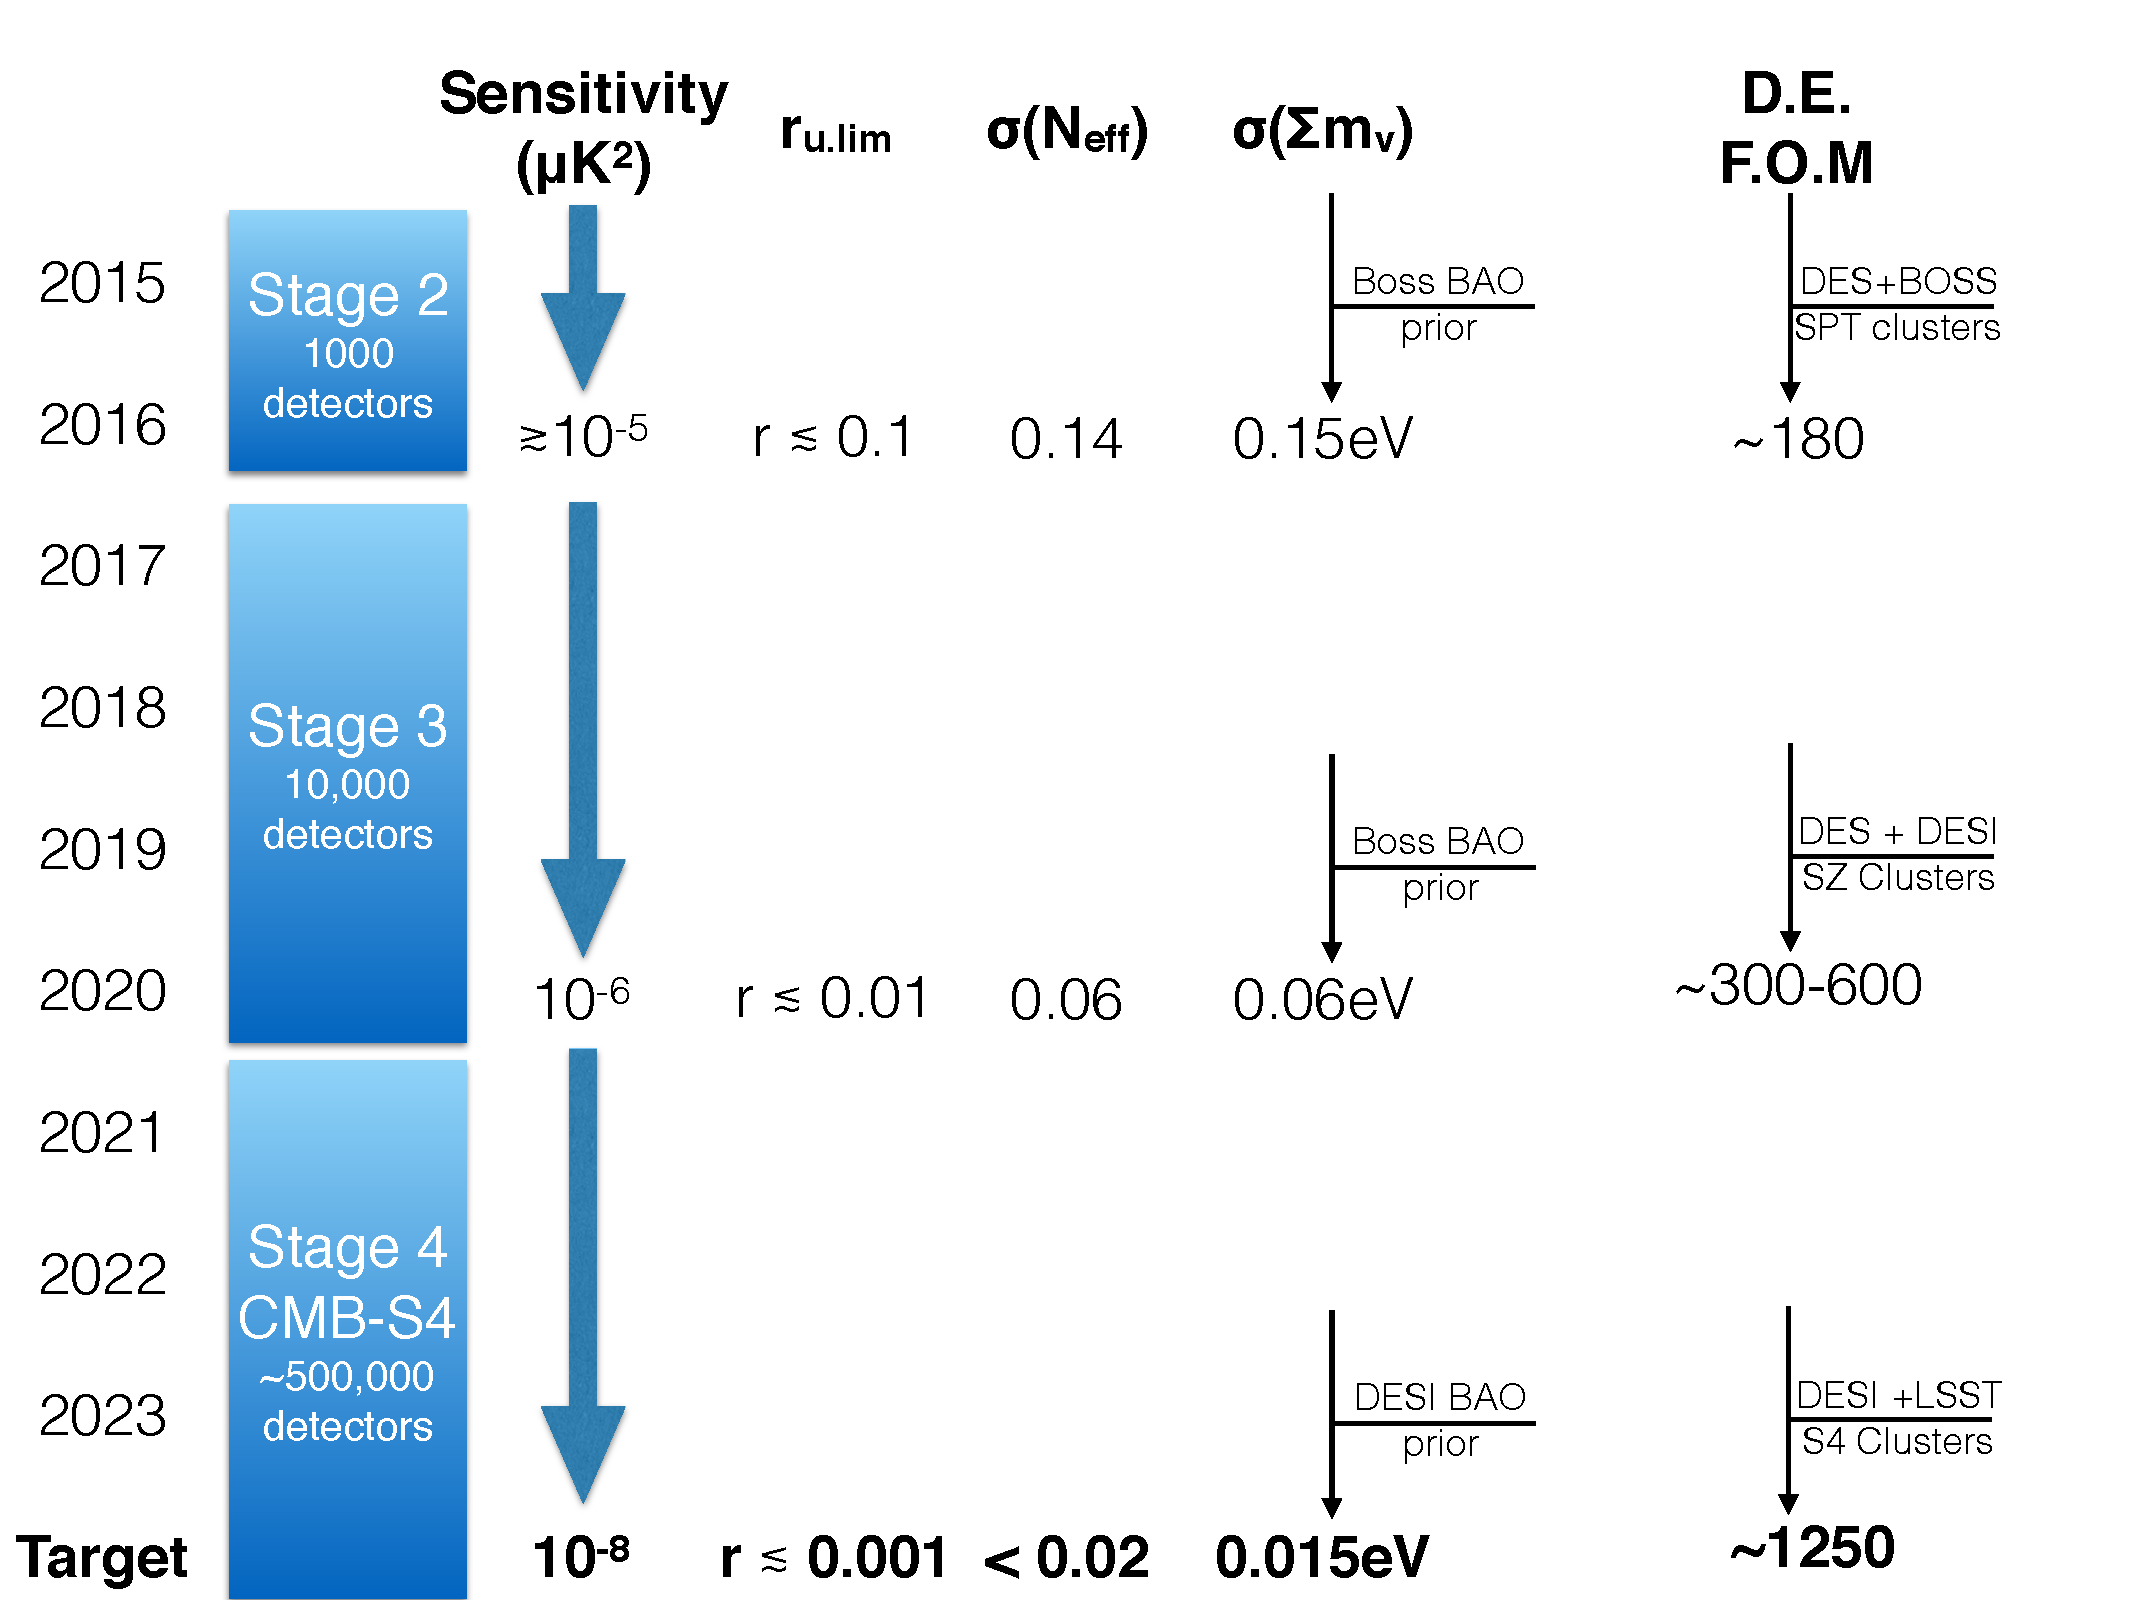
\includegraphics[width=0.95\textwidth]{Intro/Fig-FlowChart1_v1.pdf}
\caption{Schematic timeline of evolution of Stage 3 and CMB-S4 
sensitivity in $\mu$K$^2$ and the expected improvement in a few of the key cosmological parameters.}
\label{fig:science_timeline-intro}
\end{figure}

Finally, in Fig.~\ref{fig:flowchart} we show how the scientific findings (yellow), the technical advances (blue) and satellite selections (green) would effect the science goals, survey strategy and possibly the design of CMB-S4.  [Figure to be updated]

\begin{figure}[ht]
\centering 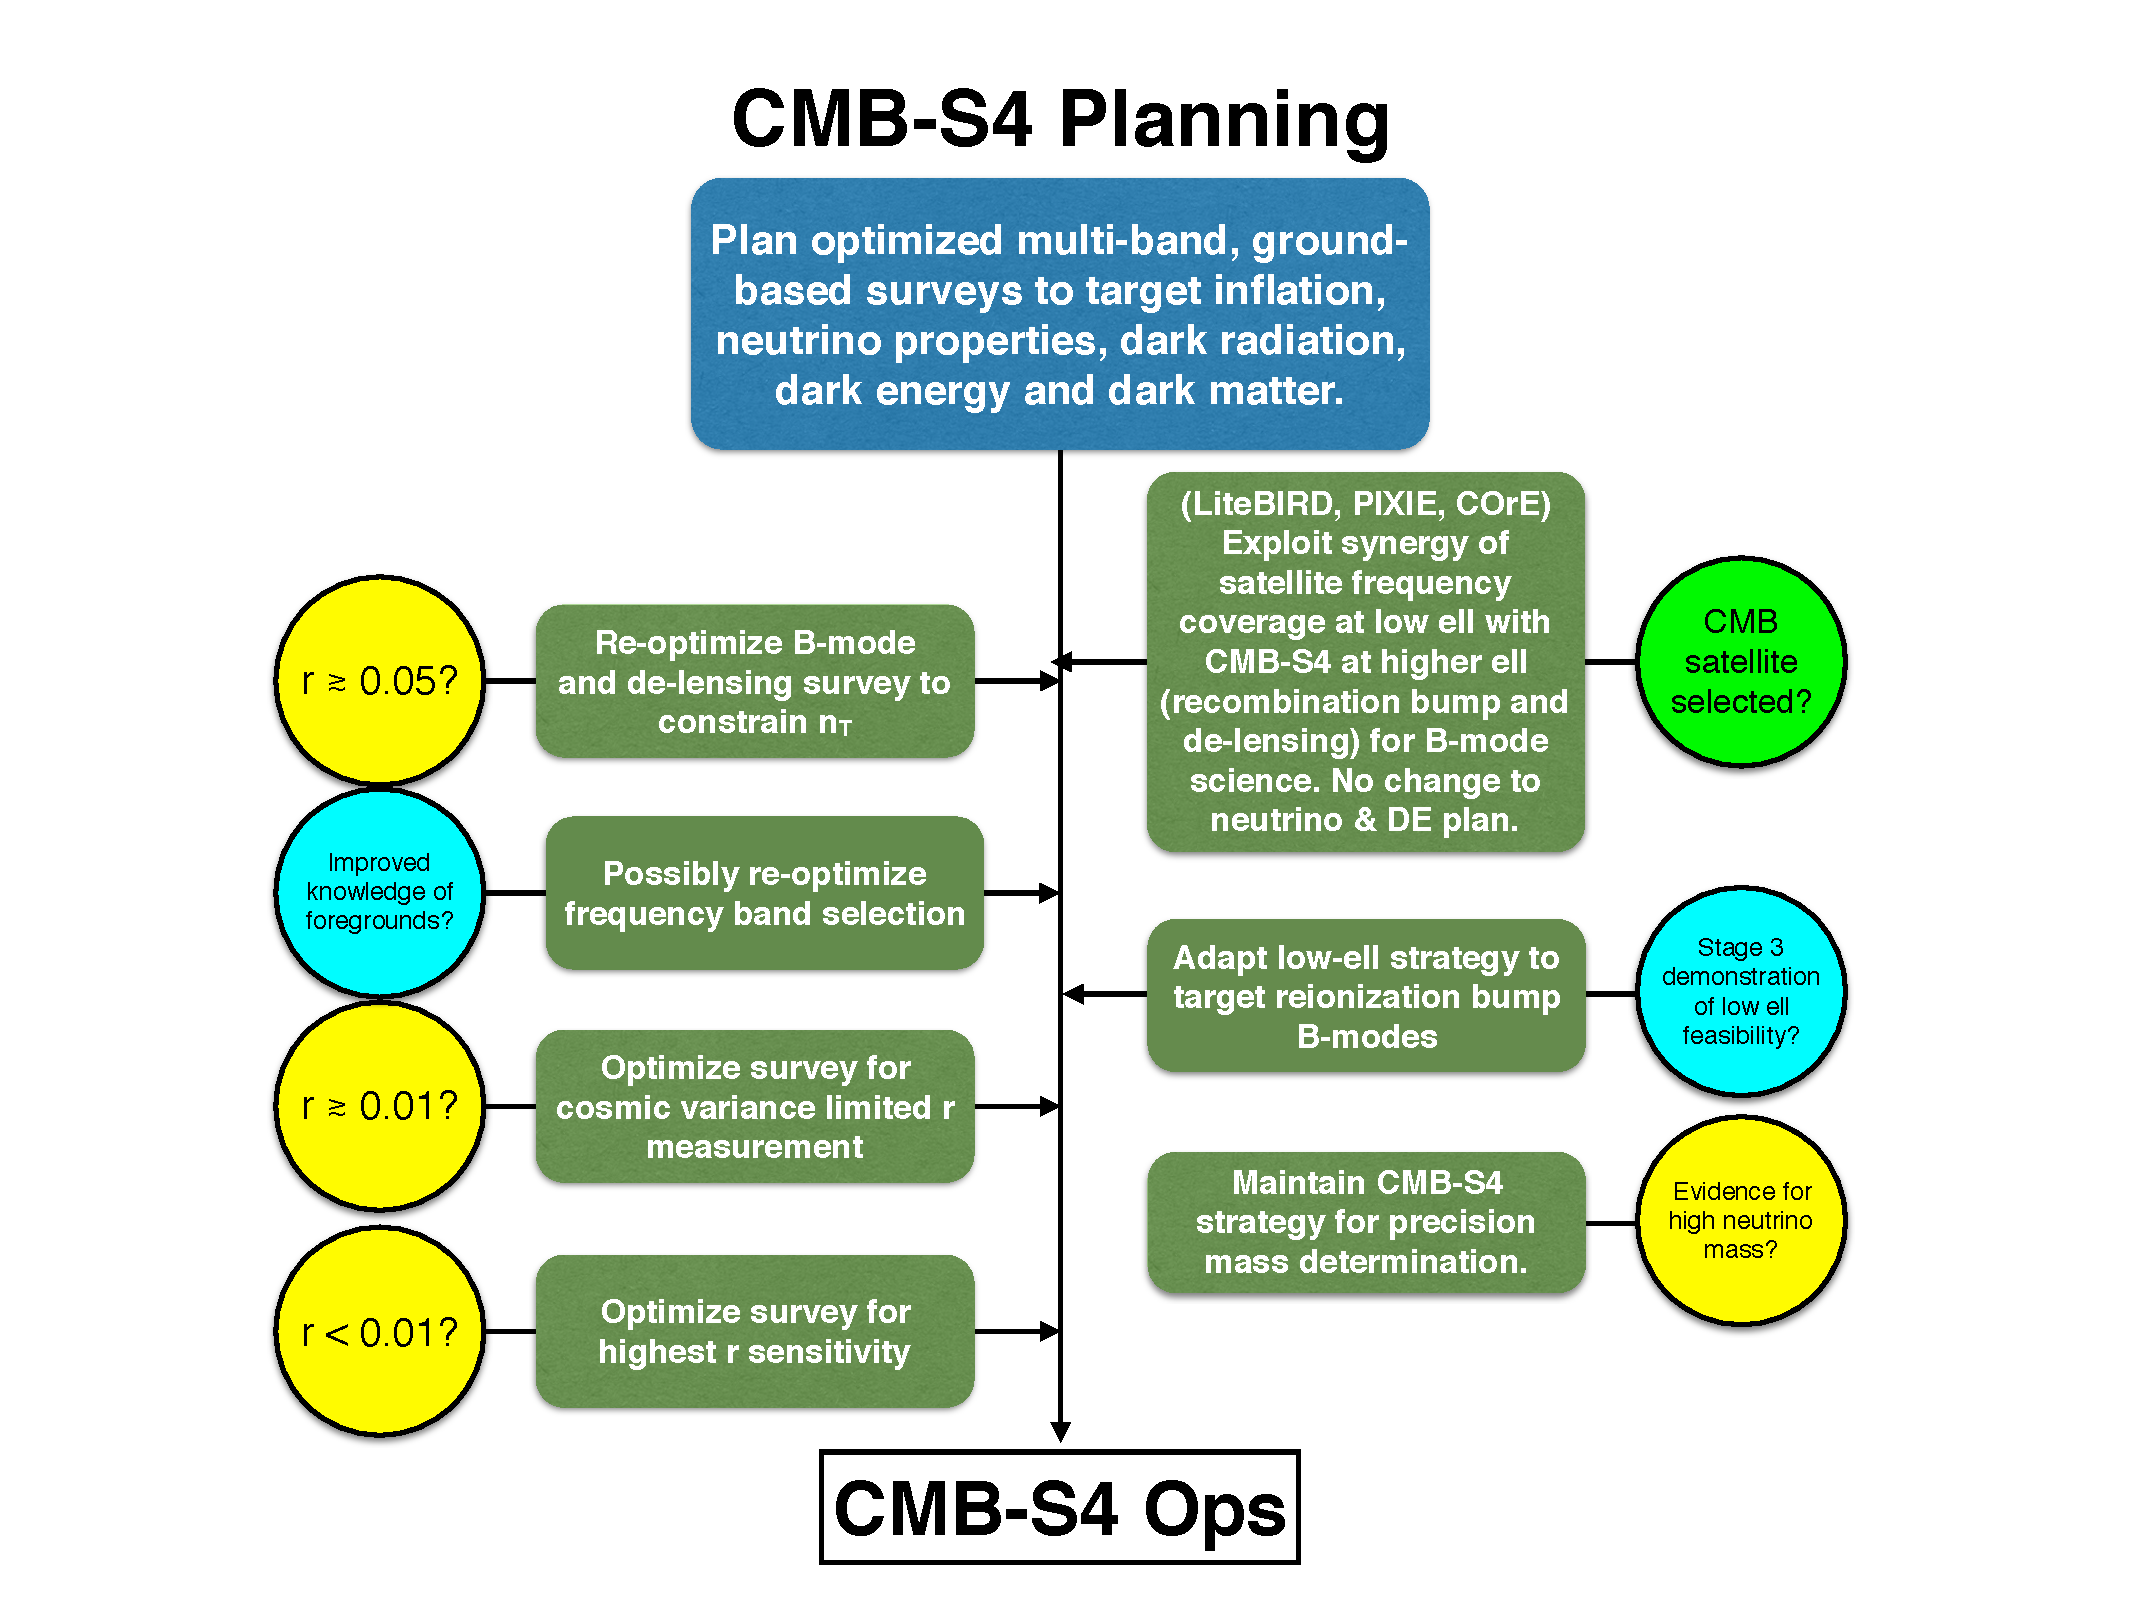
\includegraphics[trim=1in 0in 1.2in 0in, clip, width=1.0\textwidth,]{Intro/Fig-FlowChart2_v1.pdf}
\caption{Schematic flow chart showing how the scientific findings (yellow), the technical advances (blue) and satellite selections (green) would effect the science goals, survey strategy and possibly the design of CMB-S4 (green boxes) [Figure to be updated] }
\label{fig:flowchart}
\end{figure}



%\bibliography{cmbs4}

%%
%% Populate the .bib file with entries from SPIRES Bibtex (preferred)
%% or ADS Bibtex (if no SPIRES entry).
%%  SPIRES will also supply the CITATION line information; please include it.
%%


